\section{Performance Evaluation}

An Audio Plugin runs is an environment with many other components, sharing CPU resources. Processing of audio data must be completed withing descreet time intervals dictated by the audio hardware and some setting the user can configure. Typical audio sampling frequencies are 44.1kHz, 48kHz, 88.2kHz and 96kHz. Using 44.1kHz as an example, this means that all the calculations required for a single sample must be completed within 0,023 ms. Interrupts would be recieved from the audio hardware at intervals of 0.023ms as well, and this would put too much of a strain on the Operating System of the CPU though. Instead, requests for new audio data are bundled into buffers of samples. The size of the buffers is a parameter that the user can modify, it's usually set at 512 samples, but can be as low as 16 samples.

Increasing the buffer size, increases the amount of time that the CPU has to provide the audio data to the audio hardware, this introduces latency into the system though. A buffer size of 512 samples equates to a latency of 11.60ms. A 16 sample buffer size equates to 0.36ms.

If a single plugin requires 1.0ms to complete its processing then it will not finish in time if the buffer size is set too low. If the buffer size is just high enough, then there still might not be enough CPU resources left for other plugins to complete their tasks.

\subsection{Synchronous Performance}

This project offloads the processing to an external SBC device. However, no resources are saved if the audio plugin is blocked while it waits for the results from the SBC device. Since the external SBC devices are slower than the main CPU, the processing time will take longer. Adding the time it takes to serialise and deserialise the Datagram packet at each end will degrade performance even more.

Figure~\ref{fig:local_vs_remote} illustrates the problem in more detail.

\begin{figure}[H]
    \centering
    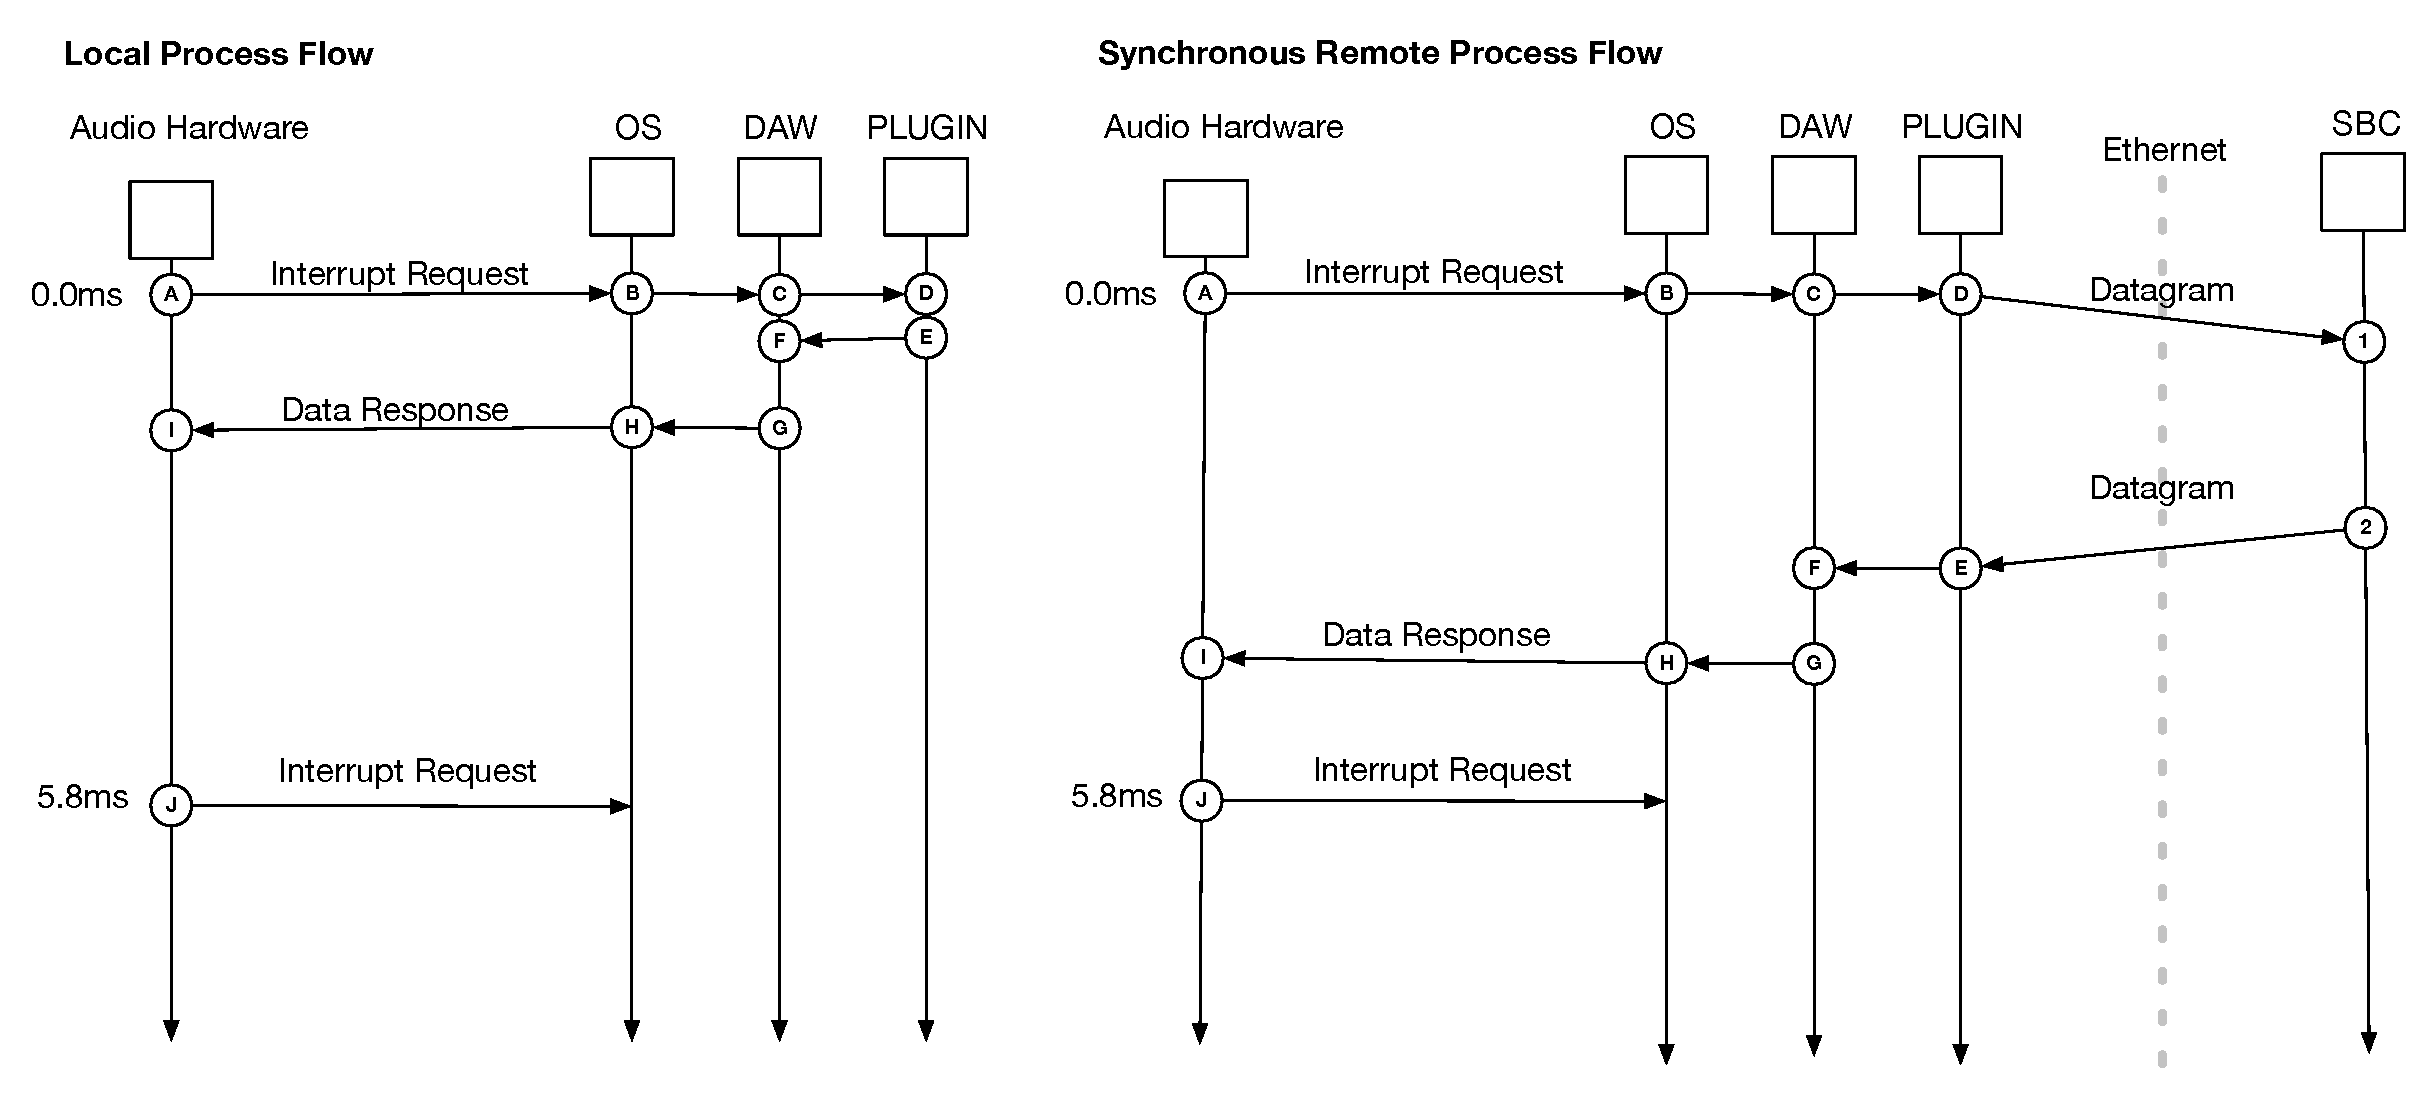
\includegraphics[width=\textwidth]{assets/conclusion/process_flow_compared.pdf}
    \caption{Local vs Remote Synchronous Processing}
    \label{fig:local_vs_remote}
\end{figure}

The example shows the audio hardware polling the operating system in intervals of 5.8 ms. This corresponds to a buffer size of 256 samples. The time interval between states D and E represents the time it takes for a plugin to process a buffer of 256 sample. The DAW can perform other audio processing functions ( including passing the buffer to other plugins ) in the interval between F and G. After states G and H the DAW and OS are free to be able to do other things, like update the GUI or check for email.

With synchronous remote processing the time between states 1 and 2 in the Remote Process Flow will add directly to the time between D and E. If that time is significantly higher than the local processing then the ability of the DAW and the OS to perform other critical tasks is impaired.

\begin{table}[H]
\begin{center}
\begin{tabular}{ |p{1.4cm}||p{1.5cm}|p{1.7cm}|p{1.7cm}|p{1.6cm}|p{1.4cm}|  }
 \hline
 buffer size    & buffer time (ms)    & rtTime (ms)   & pTime (ms)    & tTime (ms) & \% of buffer time\\
 \hline
 64             & 1.451247      & 0.574672          & 0.015857          & 0.558815      & 39.59 \\
 96             & 2.176870      & 0.575419          & 0.015851          & 0.559568      & 26.43 \\
 128            & 2.902494      & 0.59001           & 0.016519          & 0.573491      & 20.32 \\
 192            & 4.353741      & 0.67902           & 0.019013          & 0.660007      & 15.59 \\
 256            & 5.804988      & 0.707267          & 0.020352          & 0.686915      & 12.18 \\
 512            & 11.60997      & 0.707905          & 0.026348          & 0.681557      & 6.097 \\
 \hline
\end{tabular}
\end{center}
\caption{Measured Times for Synchronous Processing}
\label{tab:latency_comp}
\end{table}

Table~\ref{tab:latency_comp} shows the measured times for various buffer sizes in a remote synchronous environment that does no actually audio processing. An audio system running with a buffer size of 64 samples has 1.451ms to complete all tasks and provide the audio hardware with the resulting buffer. "rtTime" is the total round trip time. This corresponds to the time between states D and E of the Synchronous Remote Process Flow diagram in Figure~\ref{fig:local_vs_remote}. "pTime" is time interval between states 1 and 2 on the SBC device, the time spent processing the data. In this case there was no processing so this is only the measures the time spent deserialiseing and serialising the datagrams into audio and midi data. "tTime" is the "rtTime" subtracted by the "pTime" and is the packaging overhead required to send and receive data from the SBC device.

The last column, "\% of limit", shows how much time was spent in total as a percentage of the limit. At a buffer size of 64 samples 39.59\% percent of the total time available was spent by a single plugin. This does not leave much time for other processes on the CPU. For a buffer size of 512 samples the "\% of limit" value is much lower. The total system latency is slightly higher that the stated 10ms maximum though, and the synchronous design has not reduced the processing load on the CPU at all.


\subsection{Asynchronous Performance}

Instead of waiting for a response from the SBC device as in the synchronous method described above the asyncronous
method checks if a response is available, if so process it, if not immediately return. The initial request for
audio data would return empty, but by the time the second buffer is requested, the first respose from the SBC device
might have returned. In both cases the only time spent by the audio plugin itself is the time is takes to serialise and
send the data, and to receive and deserialise the data. These are the intervals between the states D and E
and M and N represented in the figure~\ref{fig:async_remote}

\begin{figure}[H]
    \centering
    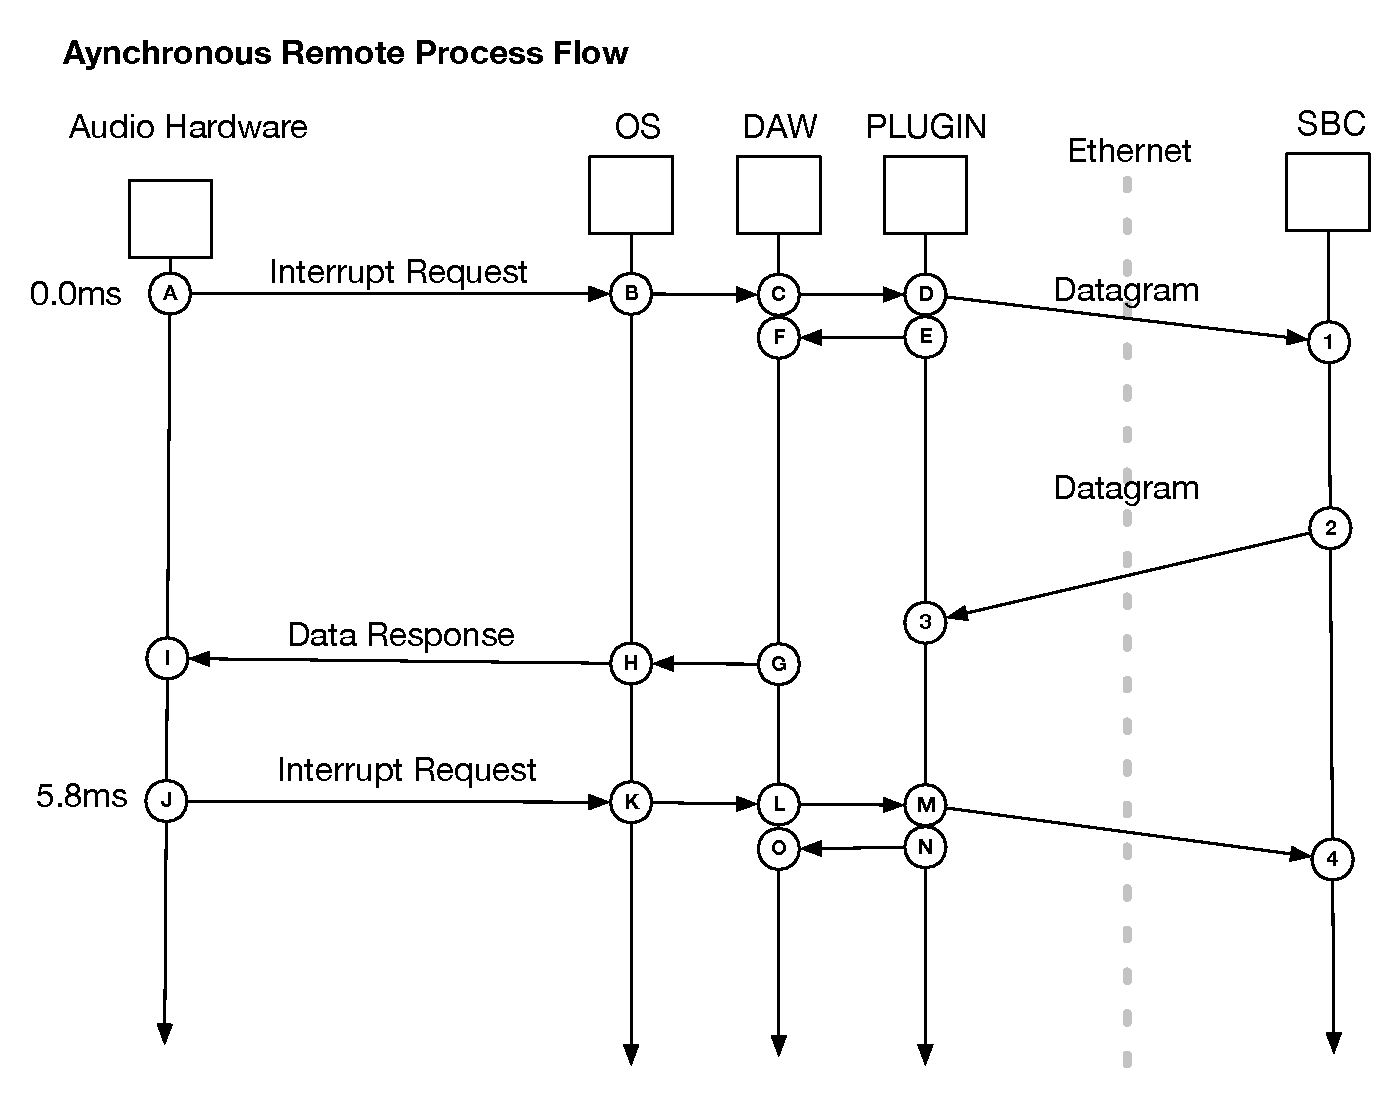
\includegraphics[width=\textwidth]{assets/conclusion/async_flow.pdf}
    \caption{Local vs Remote Synchronous Processing}
    \label{fig:async_remote}
\end{figure}

\begin{table}[H]
\begin{center}
\begin{tabular}{ |p{1.4cm}||p{1.5cm}|p{1.7cm}|p{1.7cm}|p{1.6cm}|p{1.4cm}|  }
 \hline
 buffer size    & limit (ms)    & rtTime (ms)   & pTime (ms)    & tTime (ms) & \% of limit\\
 \hline
 64             & 1.451247      & 0.031683          & 0.015633          & 0.016050      & 2.18 \\
 96             & 2.176870      & 0.046585          & 0.016076          & 0.030509      & 2.14 \\
 128            & 2.902494      & 0.034745          & 0.016712          & 0.018032      & 1.19 \\
 192            & 4.353741      & 0.052279          & 0.018800          & 0.033478      & 1.20 \\
 256            & 5.804988      & 0.065752          & 0.019646          & 0.046105      & 1.13 \\
 512            & 11.60997      & 0.062939          & 0.019708          & 0.043230      & 0.54 \\
 \hline
\end{tabular}
\end{center}
\caption{Measured Times for Asynchronous Processing}
\label{tab:latency_async}
\end{table}